\chapter{NOTES AND STUFF}

This appendix is for the group members to see how to code basic \LaTeX{} functions.
%%%%%%%%%%%%%%%%%%%%%%%%%%%%%%%%%%%%%%%%%%%%%%%%%%%%%%%%%%%%%%%%%%%%%%%%%%%%%%%%%%%%%%%%%%%%%%%%%%%%%
\section{Insert a figures/picture}
Remember that you need to convert to .eps if the picture to a vectorpicture before you upload it to the image folder in the svn drive. This can be done using \url{www.go2convert.com}.\\ % <- these \\ means newline

The code for including the figure is listed here:

\begin{figure}[!h]
  \centering
  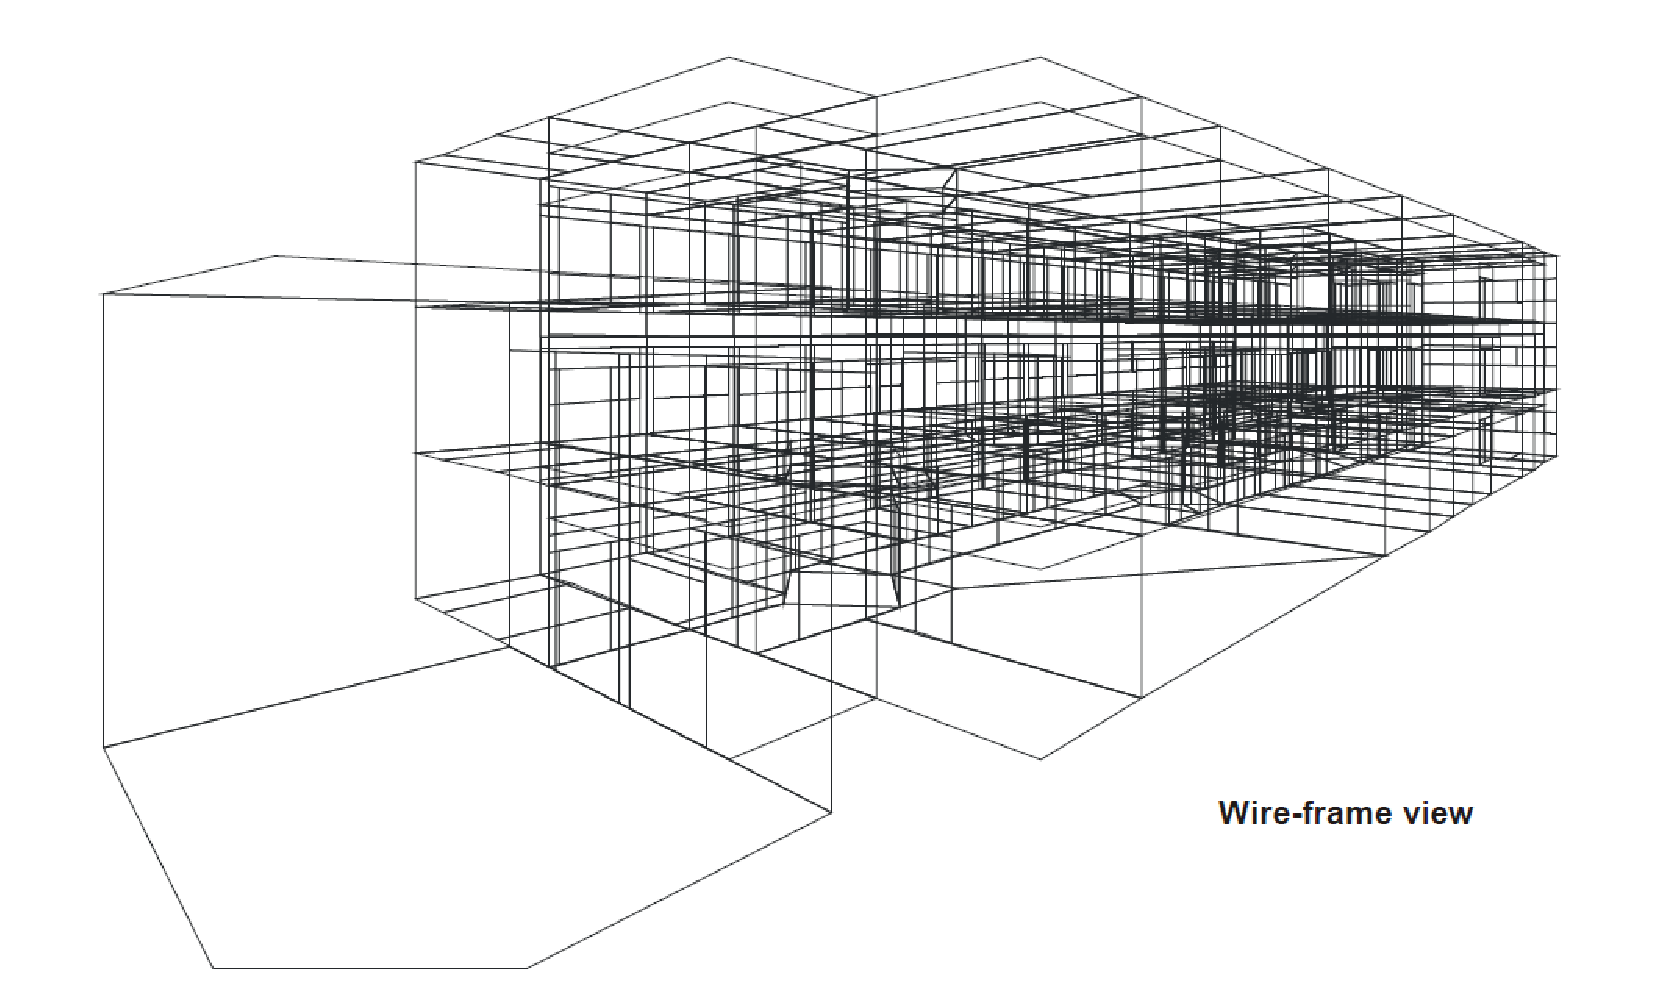
\includegraphics[width=4cm]{FrontPage.eps}
  \caption{Sample image.}
  \label{fig:REMEMBER_TO_CHANGE_THE_LABEL}
\end{figure}

When you need to write about the figure do like this: In \figref{fig:REMEMBER_TO_CHANGE_THE_LABEL} you see a sample image. The size of this can be set with the width=?? bracket.

This is a shot code for a figure:
\fig[keepaspectratio=true,width=4cm]{FrontPage.eps}{Sample image.}{fig:REMEMBER_TO_CHANGE_THE_LABEL2}

%%%%%%%%%%%%%%%%%%%%%%%%%%%%%%%%%%%%%%%%%%%%%%%%%%%%%%%%%%%%%%%%%%%%%%%%%%%%%%%%%%%%%%%%%%%%%%%%%%%%%
\section{Making a list}

To make a list with points do like this:
\begin{pitemize}
\item $P_{TX}$: Note the greenstuf in the code for this line, this is how you do math
\item Another point
\end{pitemize}

With numbers:
\begin{penumrate}
\item $P_{TX}$: Note the greenstuf in the code for this line, this is how you do math
\item Another point
\end{penumrate}

%%%%%%%%%%%%%%%%%%%%%%%%%%%%%%%%%%%%%%%%%%%%%%%%%%%%%%%%%%%%%%%%%%%%%%%%%%%%%%%%%%%%%%%%%%%%%%%%%%%%%
\section{How to write math}
If one is to write normal math expression inline then just use the dollar $style$. If you need a equation then use the following:

\begin{flalign}
&&	c_{i} =& \frac{\sum \sqrt{\left(X_{i}-X_{j}\right)^{2}+\left(Y_{i}-Y_{j}\right)^{2}}}{\sum h_{i}}	& [\SI{}{\meter}] &\label{eq:REMEMBER_TO_CHANGE_THE_LABEL3} \\
&&	dist_{ij} =& \frac{(t_4-t_1)-(t_3-t_2)}{2} \cdot v	& [\SI{}{\meter}] & \label{eq:REMEMBER_TO_CHANGE_THE_LABEL4}
\end{flalign}

The when you need to make a references to the equation you can just do like this: In \equref{eq:REMEMBER_TO_CHANGE_THE_LABEL3} it is seen that... And in \equref{eq:REMEMBER_TO_CHANGE_THE_LABEL4} it is seen that... \\

It is important always to use the right SI-unit (See: \secref{sec:SIunit}) ! Mark this in the last bracket\\
Remember not to remove the \texttt{\&} symbols in the code, these control the spacing. 

%%%%%%%%%%%%%%%%%%%%%%%%%%%%%%%%%%%%%%%%%%%%%%%%%%%%%%%%%%%%%%%%%%%%%%%%%%%%%%%%%%%%%%%%%%%%%%%%%%%%%
\section{Use the right SI-unit} \label{sec:SIunit}
We are engineers and therefore we only use correct SI-units. This is easy in \LaTeX{} as there is a function for this and it works all over. You do like this:\\

If we need to write something in meters then do this: \SI{10,00}{\meter} or \SI{10.00}{\meter}, as seen in the code first bracket is the number, and you can use dot or comma it will be correct in the pdf as the SI function controls this.  Some other examples: \SI{0.01}{\micro\watt} / \SI{250}{\milli\watt} / \SI{285.517}{\milli\meter} / \SI{2100}{\mega\hertz} /\SI{}{\decibelm}. Lastly here is one where we have the per symbol and want i ``pretty'' as you know i like; \SIf{}{\meter\per\second} otherwise it will be; \SI{}{\meter\per\second}

%%%%%%%%%%%%%%%%%%%%%%%%%%%%%%%%%%%%%%%%%%%%%%%%%%%%%%%%%%%%%%%%%%%%%%%%%%%%%%%%%%%%%%%%%%%%%%%%%%%%%
\section{Use references wisely} \label{sec:refs}
When working in latex one of the most important features is that references is generic. Therefore it is important to use these correct. We are using the labels to reference to this and as you may have notice in the code the first part of the label refers to what the label is attached to. eg. ``sec:'' for a section and ``eq:'' for a equation. We use different references as to where it is used and to what it refers, here is some examples:\\

(See \chref{ap:basiclatex}) will give you ``See chapter A'' \\ % yes it should be {ch:something} but i just use the other label as a exampel here.
(See \secref{sec:SIunit}) will give you ``See section A.4 (p.13)'' \\
(See \figref{fig:REMEMBER_TO_CHANGE_THE_LABEL2}) will give you ``See figure A.2 (p.12)'' \\
(See \equref{eq:REMEMBER_TO_CHANGE_THE_LABEL4}) will give you ``See equation A.2 (p.13)'' \\
(See \apref{ap:basiclatex}) will give you ``See appendix A (p.12)'' \\

And as you may already notice this change as the document evolves and therefore what I have put in with hardcode is already wrong. But the generic code using the correct labels and ref-types is always referring to the correct place.\\

If you need to make a reference to something and there is no label yet, then always put it on the chapter/section header or similar as this is then the place all of us can look for it. Good practice is always to make a label then others can use this even if you do not need it yourself.

%%%%%%%%%%%%%%%%%%%%%%%%%%%%%%%%%%%%%%%%%%%%%%%%%%%%%%%%%%%%%%%%%%%%%%%%%%%%%%%%%%%%%%%%%%%%%%%%%%%%%
\section{Making a table} 
\ptable{| p{10cm} | p{8cm} |}{ %
Property 							&	Description 												\\ \hline
Gain of received power 		        &	$G_r = 1$											        \\ \hline
Gain of transmitted power 	        &	$G_t  =  1$										            \\ \hline
Frequency							&	\textit{f} in \SI{}{\hertz}	    							\\ \hline
Propagation speed of signal			& 	$c$ in \SIf{}{\meter\per\second}                            \\ \hline	
Power transmitted 			        &	$P_{t(dBm)}$ in \SI{}{\decibelm} 	                        \\ \hline
}{Free-Space Model properties}{tab:environment}

The properties needed to define the Free-Space Model is listed in \tref{tab:environment}.  

\section{How to insert Matlab code in latex}
We use the folder \texttt{code} in the SVN folder. Therefore latex can extract and display code in the worksheets without the need of copying anything. \\

An example of this is seen below:
\code{language=Matlab,caption = Friis propagation model,label=cl:envfreespace,linerange={1-8},firstnumber=1}{code/initPropaFriis.m}

Note that there is multiple parameters which have to be set: \\
language        = Matlab                          (The language of the code)                 \\
caption         = What ever the caption should be                                            \\
label           = cl:REMEMBER LABEL               (Give a unique label name)                 \\
linerange       = {1-8}              (Set the linerange of code you want to be shown)        \\
firstnumber     = 1                  (Set the first linenumber shown in the latex file)      \\

A reference to the code can be done like this; As seen in \cref{cl:envfreespace}...